\documentclass[12pt,a4paper]{article}

% Packages
\usepackage{amsmath}
\usepackage{amsfonts}
\usepackage{amssymb}
\usepackage{graphicx}
\usepackage[margin=1in]{geometry}
\usepackage{enumitem}
\usepackage[hidelinks]{hyperref}
\usepackage{xcolor}

% Title
\title{Homework Report for Computer Vision}
\author{Yu Xiang, Luo}
\date{\today}

\begin{document}

\maketitle

\[
	\text{Minor parts of my code take reference from }\href{https://github.com/Mike-Zheng/NTU-Computer-Vision-I-/tree/master/hw2}{\text{\textcolor{red}{this github}}}
\]
\[
	\href{https://github.com/YuXiangLo/Computer-Vision}{\text{\textcolor{blue}{You can check this github for more information}}}
\]

\section*{A Binary Image}
A naive \textbf{\texttt{for}} loop can solve it.
\[
	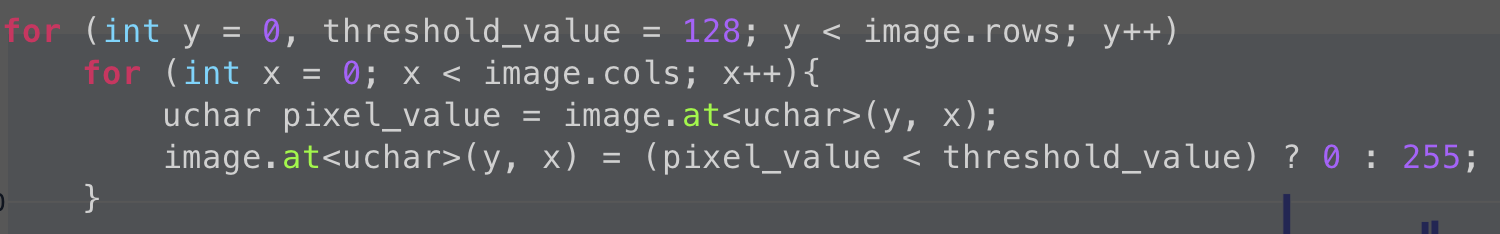
\includegraphics[width=0.9\textwidth]{./img/binary.png}
\]
\[
	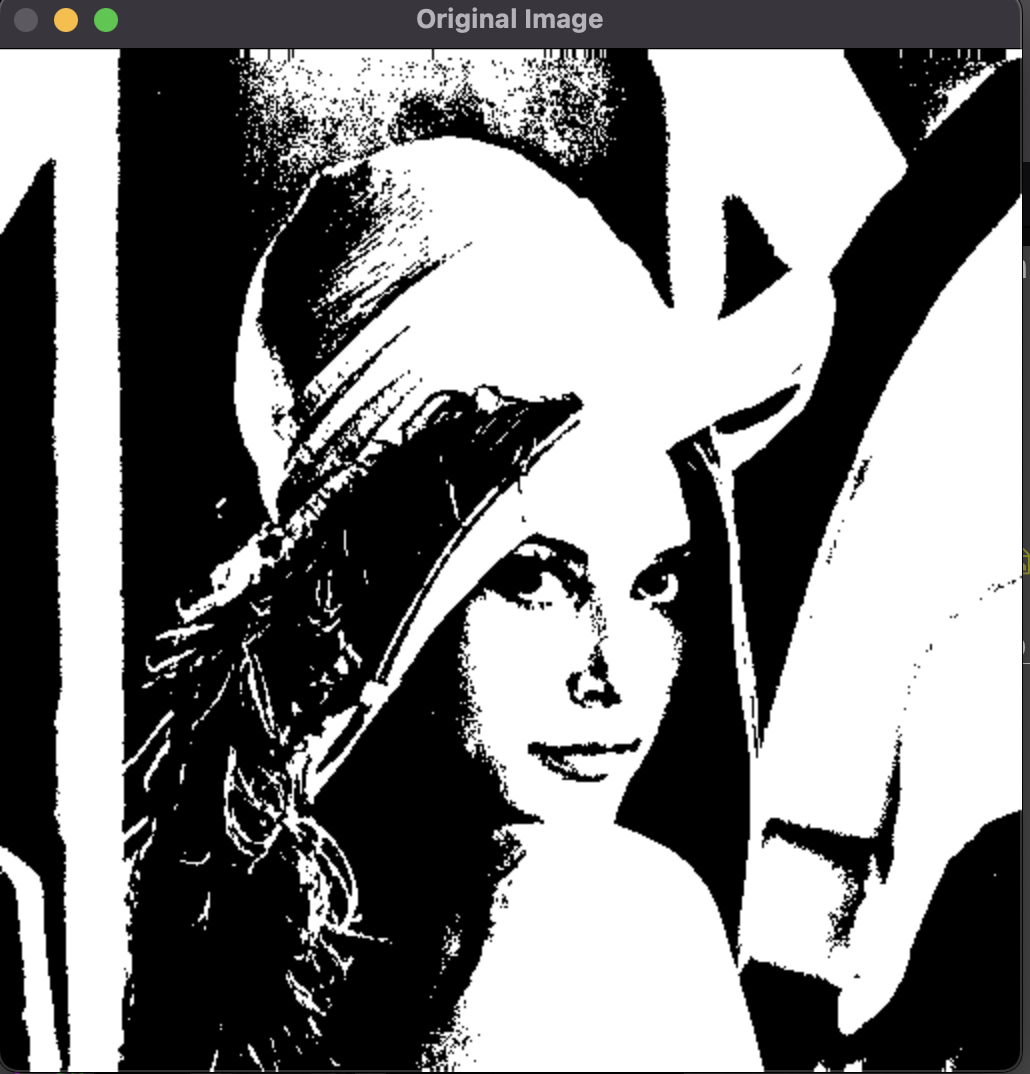
\includegraphics[width=0.7\textwidth]{./img/binaryLena.png}
\]

\newpage
\section*{Histogram}
Find the intensity at each pixel, then store it to the array \textbf{histogram}. Store the array to an csv file and use plotly to draw the histogram.
\[
	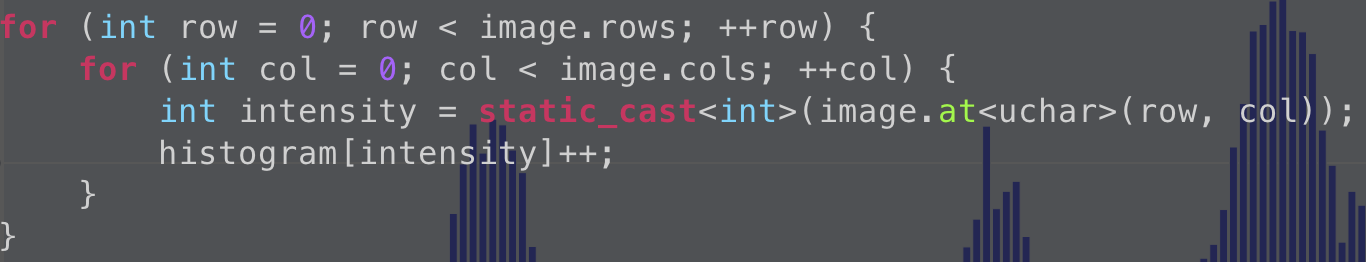
\includegraphics[width=0.9\textwidth]{./img/intensity.png}
\]
\[
	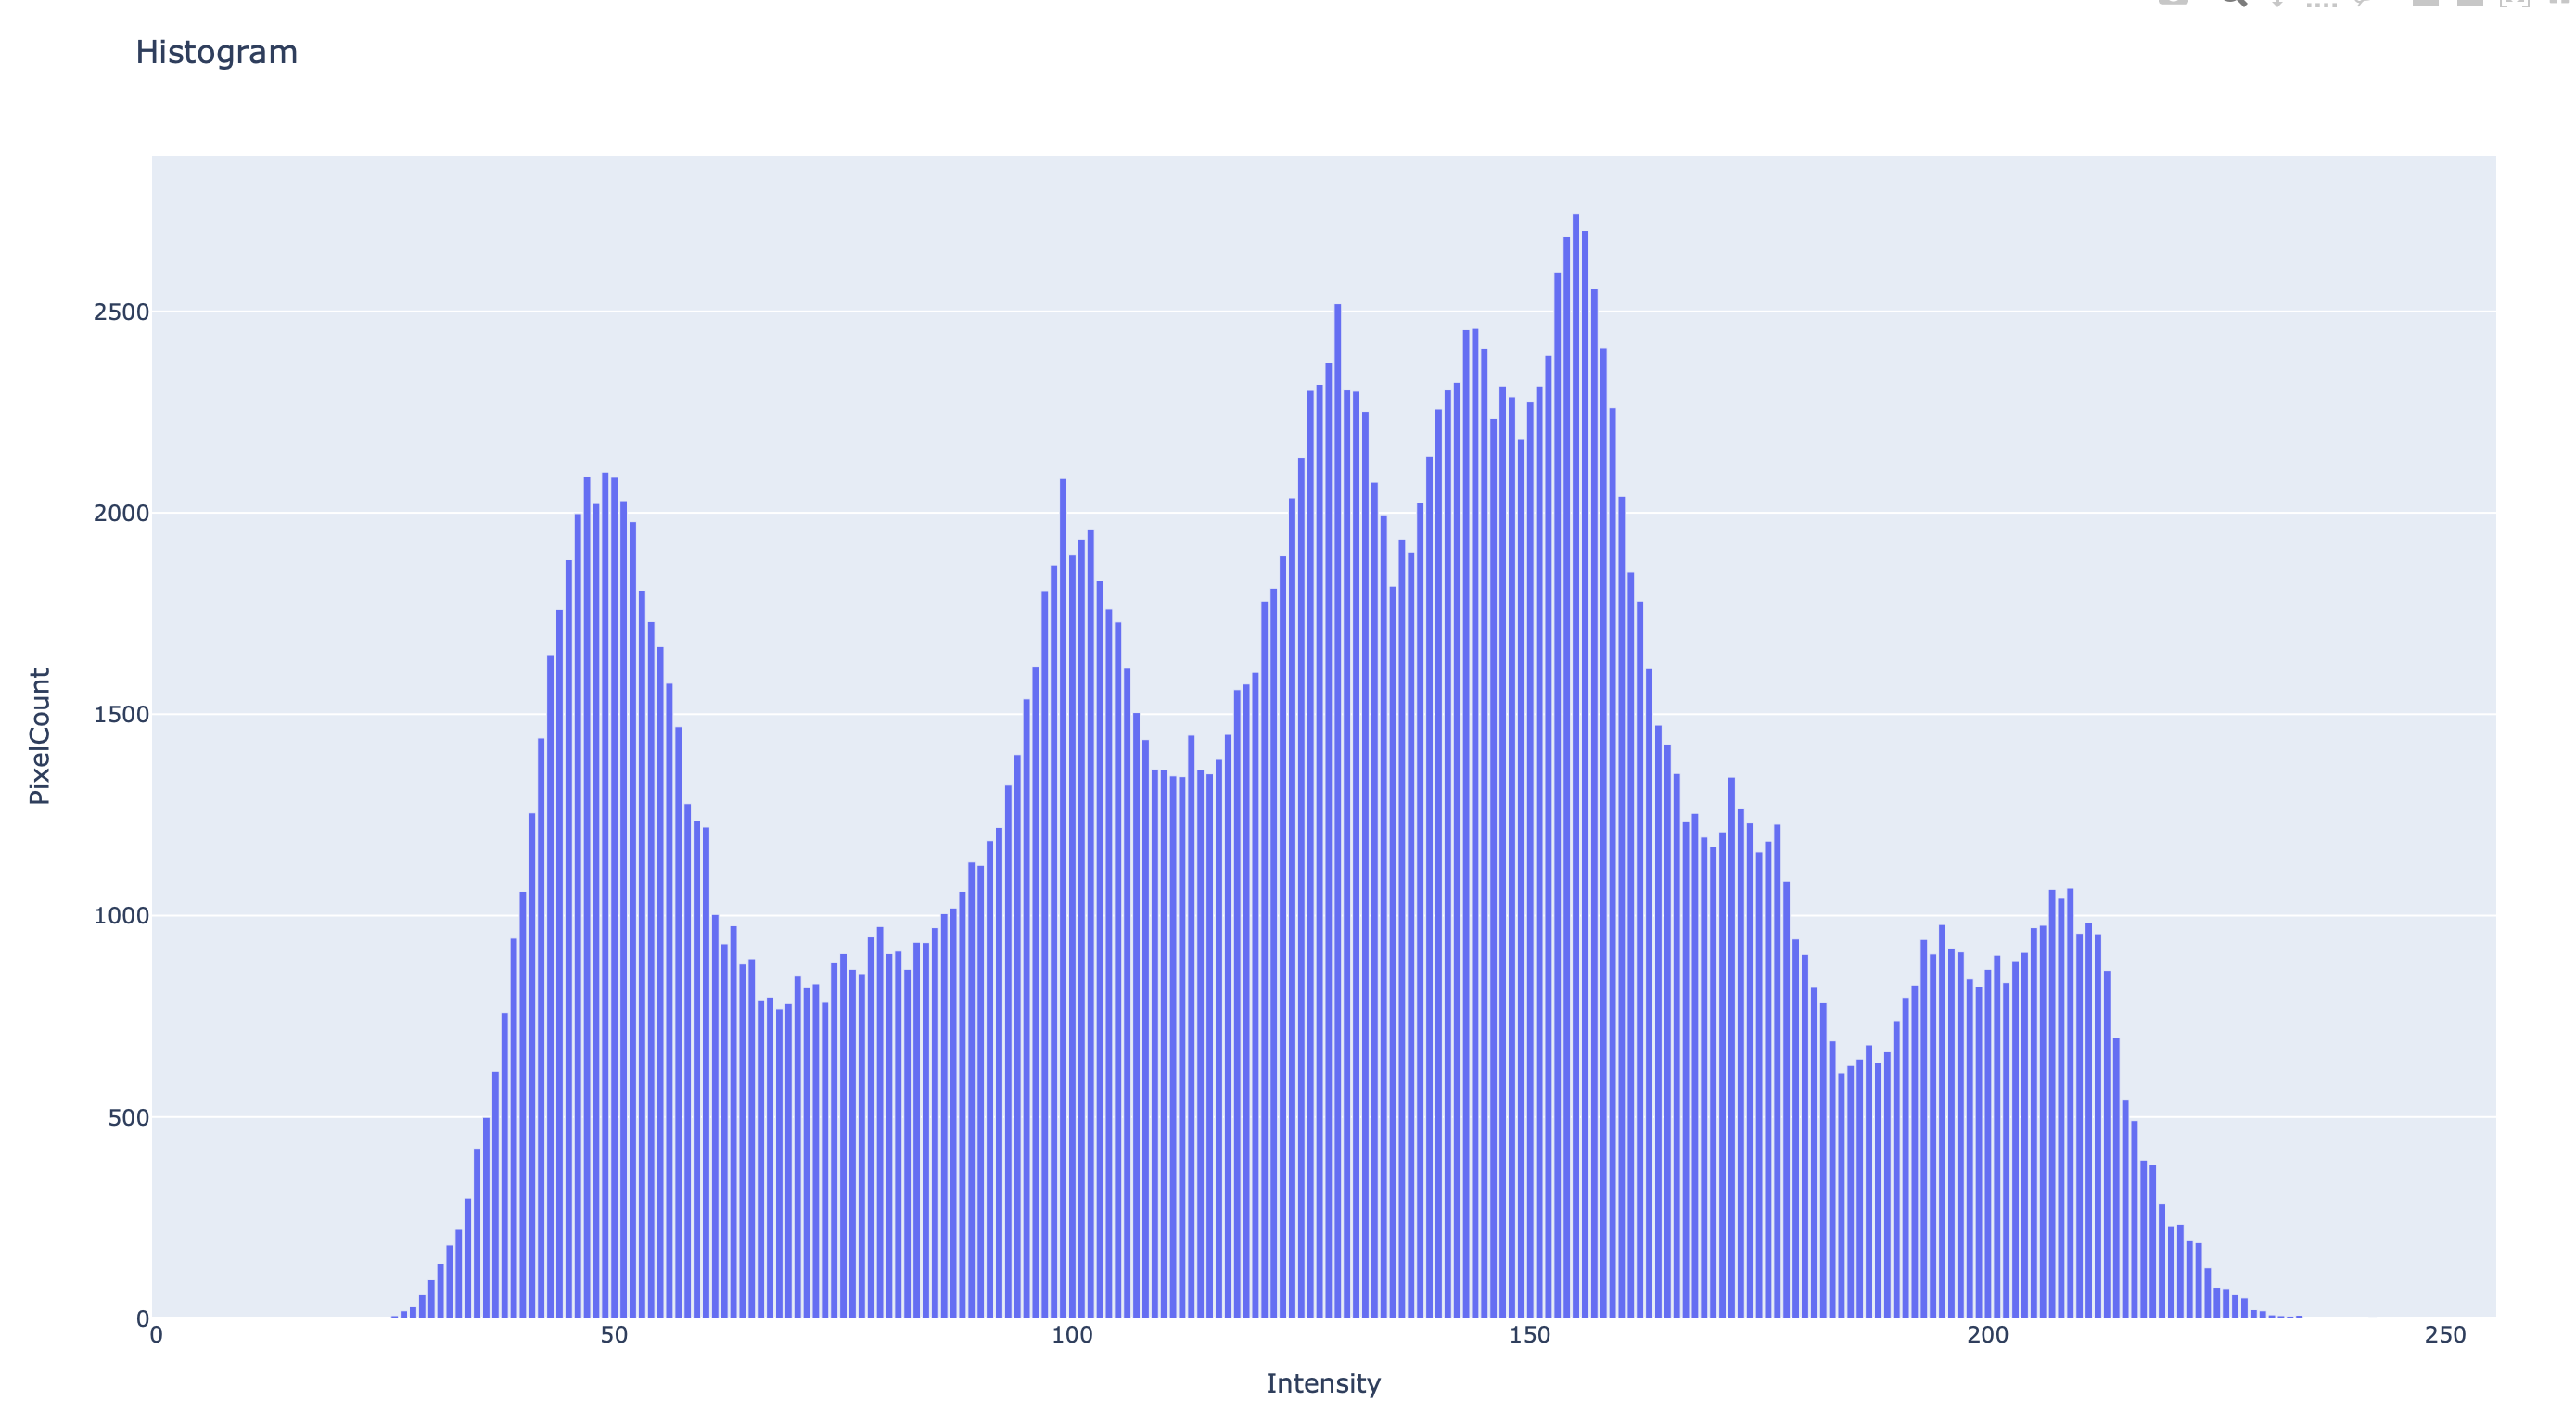
\includegraphics[width=0.9\textwidth]{./img/graph.png}
\]

\newpage
\section*{Connected Conponents – 4-connected}
Since one \textbf{cc}(connected conponent) must connect to its neighbor, so my implementation is based on this property. I'm using an array ccID to store different \textbf{cc}'s ID.
\[
	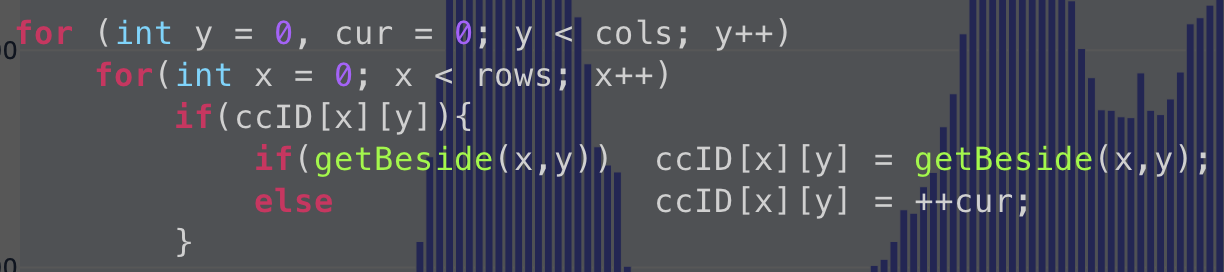
\includegraphics[width=0.9\textwidth]{./img/getBeside.png}
\]
If the pixel beside the current pixel has already been assigned a ID, then current pixel use that as its own ID, thus achieve the concept of \textbf{cc}: Pixels that connect to each is one conponents(share same ID).  
\[
	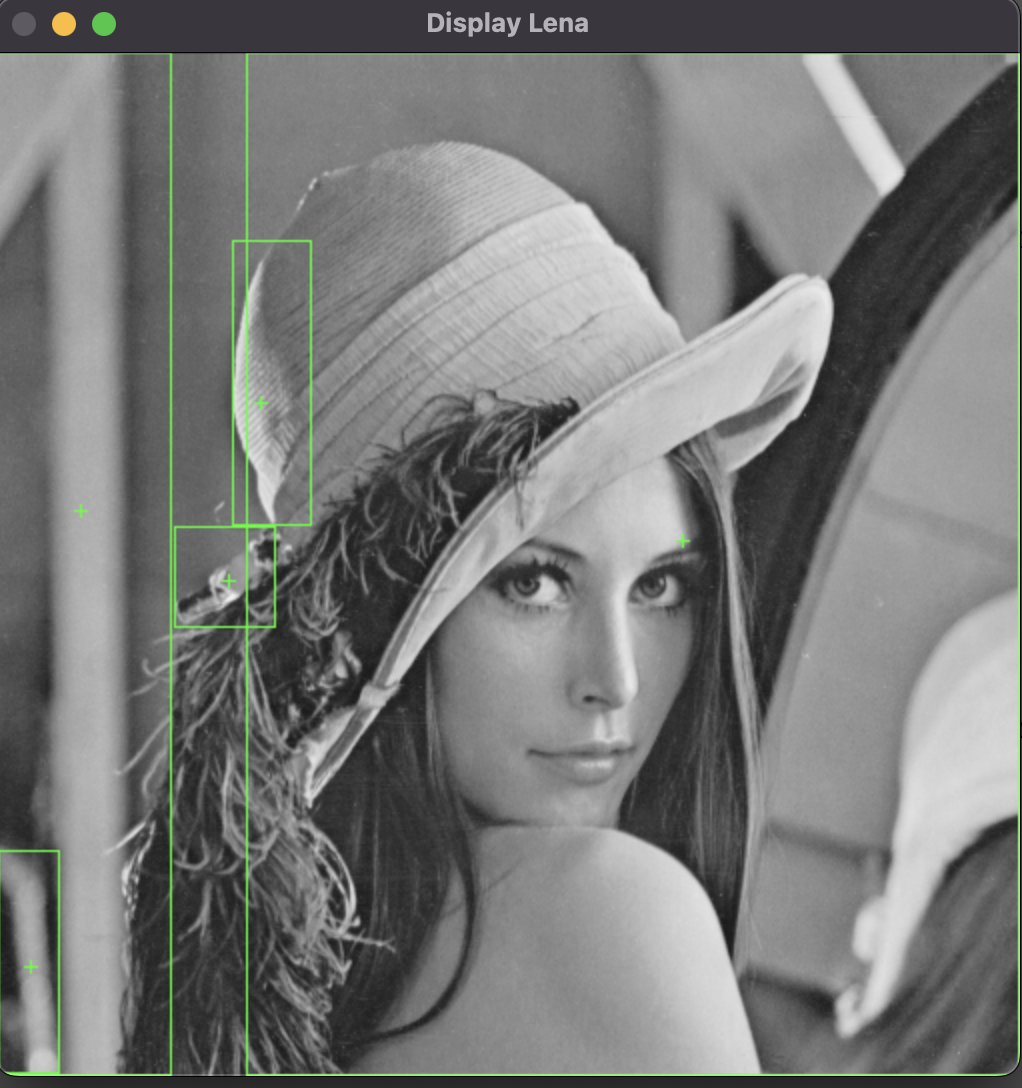
\includegraphics[width=0.9\textwidth]{./img/cc.png}
\]

\section*{Others}
For details:
\begin{enumerate}
	\item How to draw a graph: PLZ take reference to graph.py
	\item How to store histogram as csv file: PLZ take reference to histogram.cpp
	\item How to draw center and line at \textbf{cc}: Use ccID to find the leftmost, rightmost, upmost, downmost index and label them as min..., then use the function \textbf{\texttt{drawline}}, \textbf{\texttt{drawcenter}} to mark ccID as -1, then color them in the end. 
\end{enumerate}


\end{document}
